\documentclass[12pt,a4paper]{article}

\usepackage[T2A]{fontenc}
\usepackage[utf8]{inputenc}
\usepackage[russian]{babel}
\usepackage{amsmath,amssymb}
\usepackage{booktabs}
\usepackage{graphicx}
\usepackage{float}
\usepackage{hyperref}
\usepackage{geometry}
\geometry{margin=2.2cm}

\title{Отчёт по ЛР 3: Анализ Loss Landscape нейросети на CIFAR-10}
\author{Павел Тищенко}
\date{\today}

\begin{document}
\maketitle
\tableofcontents
\newpage

\section{Постановка задачи}

\subsection{Цель}
Построить и проанализировать локальное двумерное сечение функции потерь обученной CNN-модели на CIFAR-10, сравнив качество трёх квадратичных аппроксимаций поверхности.

\subsection{Формальная постановка}
Рассматривается поверхность:
\[
f(\alpha, \beta) = L(\theta + \alpha d_1 + \beta d_2),
\]
где $\theta$ --- параметры обученной модели, а $d_1, d_2$ --- случайные направления в пространстве параметров после filter-wise normalization.

Задача:
\begin{enumerate}
    \item вычислить $f(\alpha,\beta)$ на сетке в диапазоне $[-r, r]^2$;
    \item получить 1D-срезы $f(\alpha,0)$ и $f(0,\beta)$;
    \item сравнить аппроксимации $q_1, q_2, q_3$ по метрикам $RMSE$, $L_\infty$, $RelRMSE$;
    \item интерпретировать, как меняется ошибка аппроксимации при изменении радиуса.
\end{enumerate}

\subsection{Гипотеза исследования}
В малой окрестности минимума полная квадратичная аппроксимация ($q_1$) и диагональная аппроксимация ($q_2$) должны описывать поверхность точнее, чем аппроксимация на базе конечных разностей гессиана ($q_3$), чувствительная к численным эффектам.

\section{Данные и EDA}

\subsection{Источник данных}
Используется датасет CIFAR-10 (10 классов, изображения $32 \times 32$).

\subsection{EDA, релевантный задаче ЛР}
Для данной ЛР основной акцент не на табличном EDA, а на:
\begin{itemize}
    \item сбалансированности классов;
    \item визуальной проверке качества входных изображений;
    \item статистике значений пикселей после преобразований.
\end{itemize}

\begin{figure}[H]
    \centering
    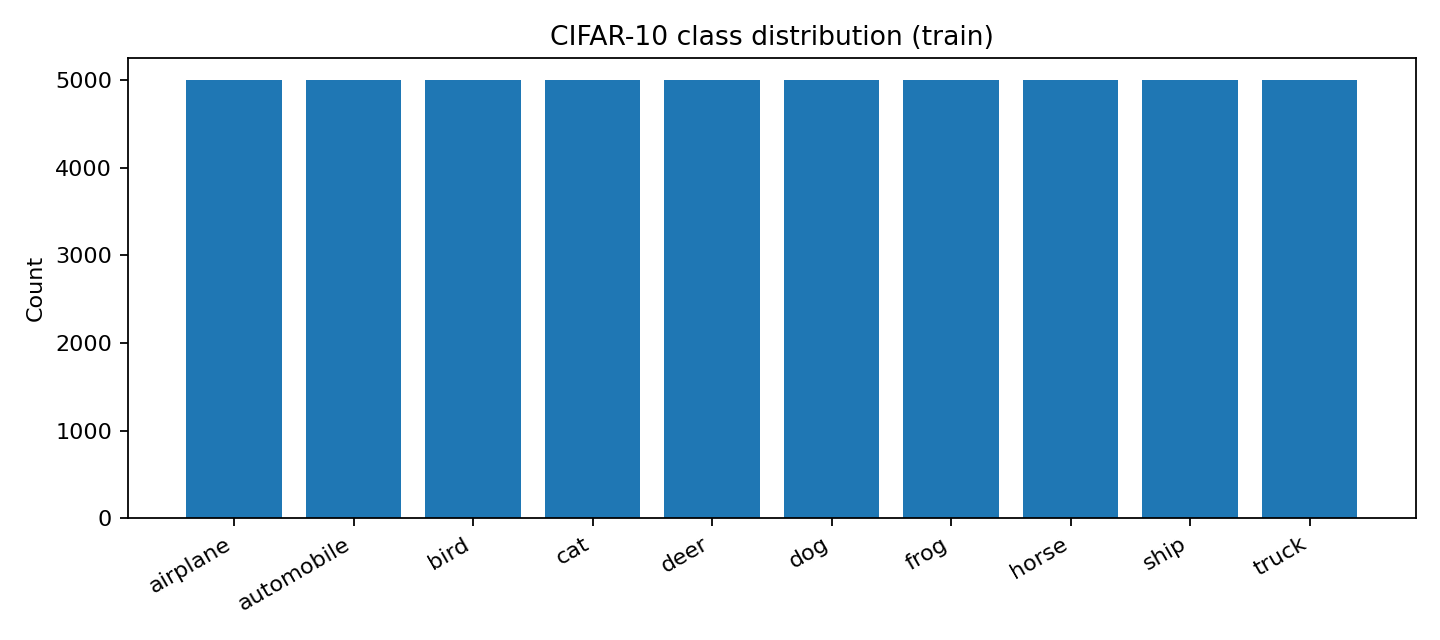
\includegraphics[width=0.75\textwidth]{figures/eda_class_distribution.png}
    \caption{Распределение классов в train-части CIFAR-10.}
    \label{fig:eda_class_dist}
\end{figure}

\begin{figure}[H]
    \centering
    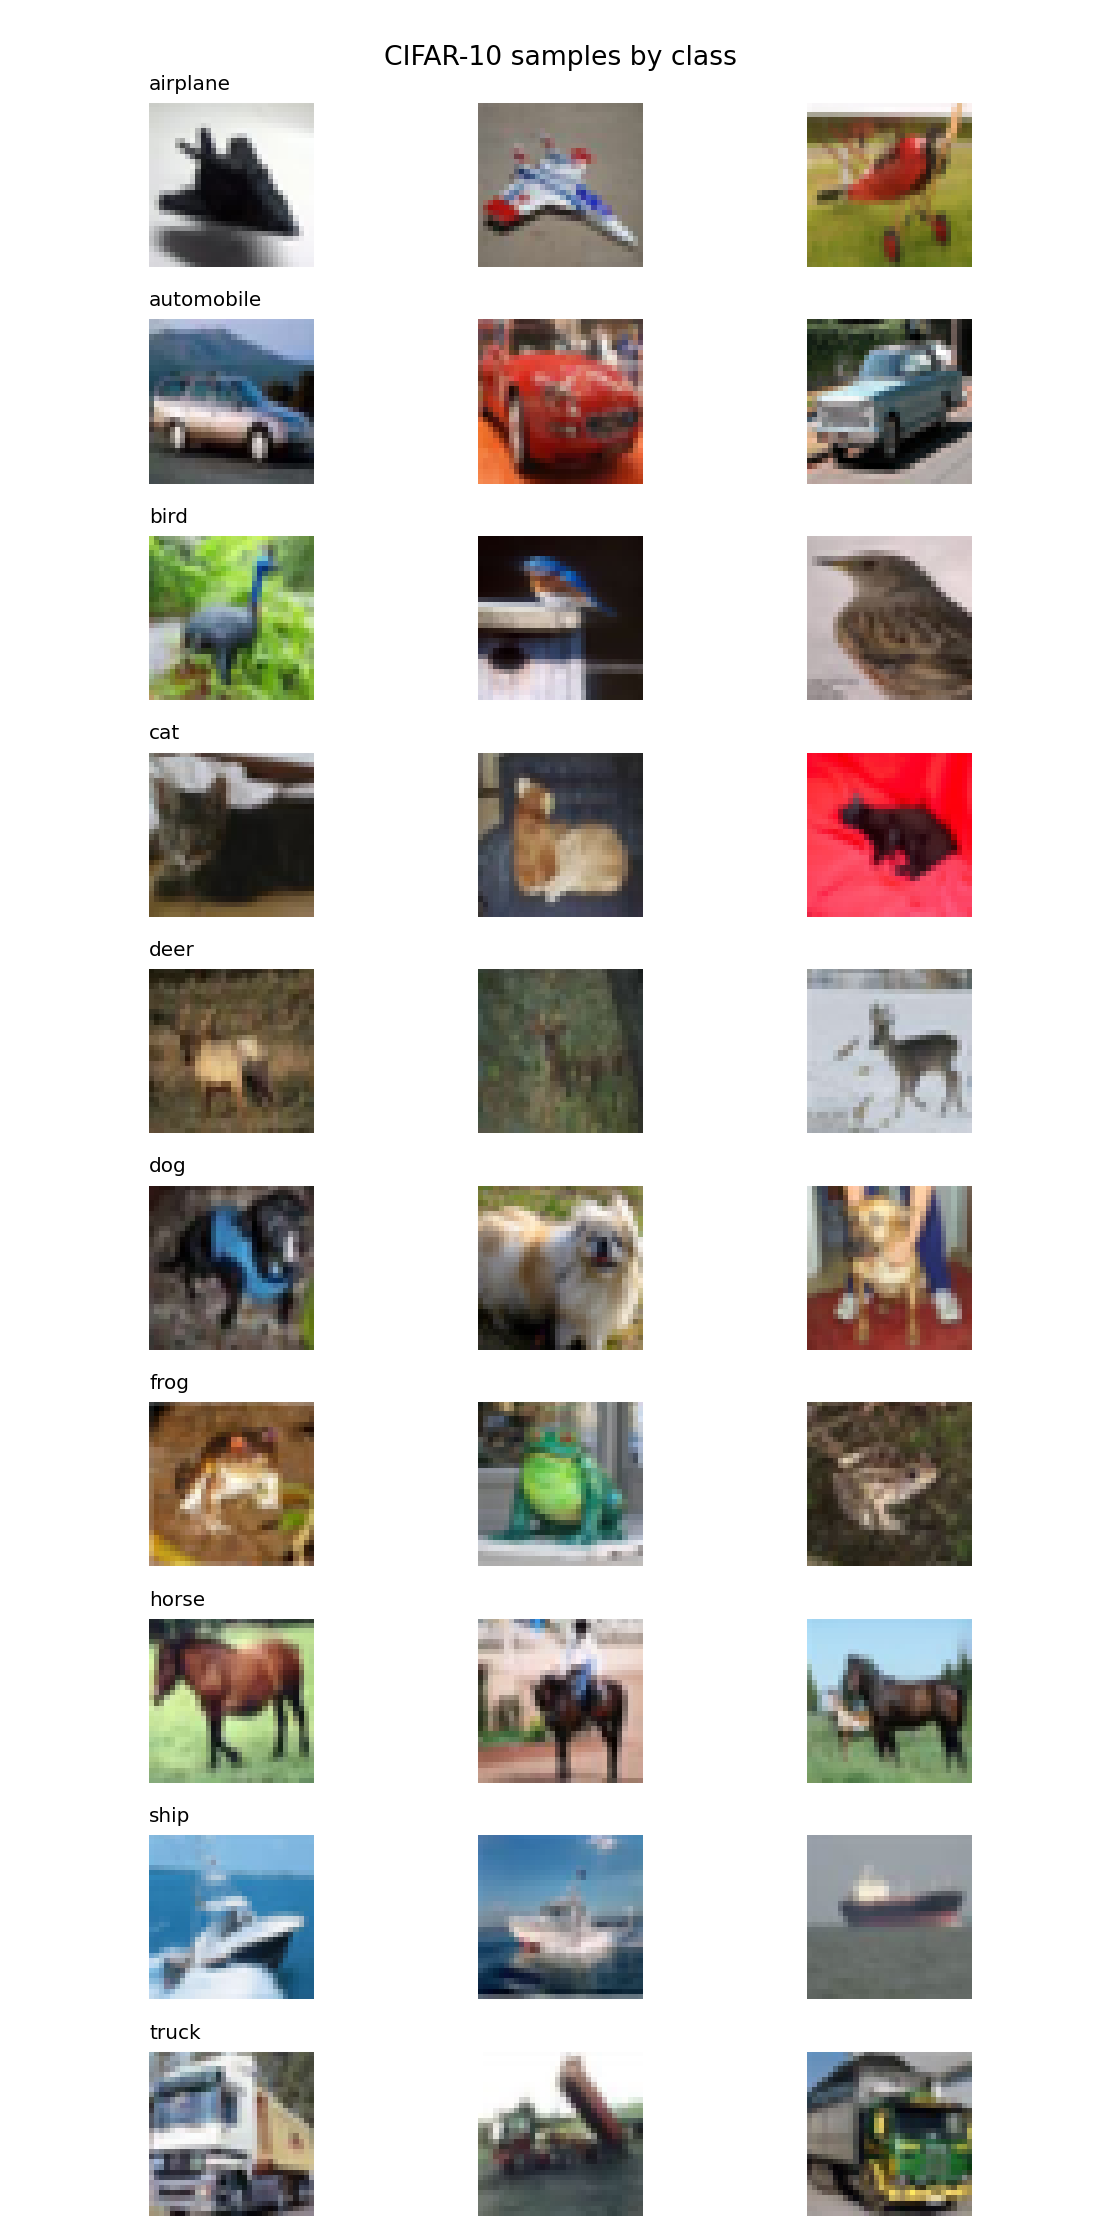
\includegraphics[width=\textwidth]{figures/eda_sample_grid.png}
    \caption{Примеры изображений CIFAR-10 (по одному/нескольким образцам классов).}
    \label{fig:eda_sample_grid}
\end{figure}

\subsection{Интерпретация}
Сбалансированность классов снижает риск смещения метрик из-за class imbalance. Для нашей задачи это важно, так как вариации в landscape должны объясняться геометрией loss и архитектурой, а не перекосом выборки.

\section{Предобработка}

Используется стандартный для CIFAR-10 набор преобразований:
\begin{itemize}
    \item train: \texttt{RandomCrop(32, padding=4)}, \texttt{RandomHorizontalFlip()}, \texttt{Normalize(mean,std)};
    \item val/test: \texttt{ToTensor()} + \texttt{Normalize(mean,std)}.
\end{itemize}

\subsection{Почему именно так}
\begin{itemize}
    \item Аугментации на train уменьшают переобучение и повышают устойчивость оценки параметров $\theta$.
    \item Единая нормализация train/val нужна для сопоставимости лосса в surface-оценке.
\end{itemize}

\subsection{Риски leakage}
В проекте нет data leakage между train и val: split берётся из официального CIFAR-10 протокола torchvision, а валидационный лосс для surface считается на test/val части без train-аугментаций.

\section{Базовая модель}

\subsection{Архитектуры}
В работе используются две архитектуры:
\begin{itemize}
    \item \textbf{model1}: residual ResNet-like;
    \item \textbf{model2}: plain-вариант без skip-connections.
\end{itemize}

\subsection{Тренировочная конфигурация}
\begin{itemize}
    \item Optimizer: SGD ($lr=0.1$, momentum $=0.9$, weight decay $=5 \cdot 10^{-4}$),
    \item scheduler: CosineAnnealingLR,
    \item epochs: 30,
    \item batch size: 128.
\end{itemize}

\subsection{Baseline-ориентиры}
Для model1 при 30 эпохах ожидаемый диапазон val accuracy: около 0.88--0.91. Это используется как sanity-check качества обученного чекпоинта перед анализом landscape.

\section{Теоретическая часть}

\subsection{Filter-wise normalization}
Для свёрточных весов направление возмущения нормируется по каждому выходному фильтру. Это уменьшает влияние масштабной неоднозначности параметров и делает визуализацию surface более интерпретируемой.

\subsection{Квадратичные аппроксимации}
\paragraph{Полная квадратика ($q_1$):}
\[
q_1(\alpha,\beta)=c+u\alpha+v\beta+\frac{1}{2}(a\alpha^2+2b\alpha\beta+d\beta^2).
\]
Коэффициенты оцениваются методом наименьших квадратов; матрица второй производной проектируется на конус положительно определённых.

\paragraph{Диагональная квадратика ($q_2$):}
\[
q_2(\alpha,\beta)=c+u\alpha+v\beta+\frac{1}{2}(a\alpha^2+d\beta^2),\quad b=0.
\]

\paragraph{Hessian FD-квадратика ($q_3$):}
\[
q_3(\alpha,\beta)=L_0+g_1\alpha+g_2\beta+\frac{1}{2}(H_{11}\alpha^2+2H_{12}\alpha\beta+H_{22}\beta^2),
\]
где $g_1,g_2$ и $H_{ij}$ оцениваются по градиенту и конечным разностям.

\subsection{Ключевая гипотеза}
При малом радиусе $r$ поверхность локально близка к квадратичной, поэтому $q_1$ и $q_2$ должны давать меньшую ошибку, чем $q_3$.

\section{Эксперименты}

\subsection{Протокол}
\begin{itemize}
    \item Модель: model1.
    \item Радиусы: $r \in \{0.1, 0.25, 0.5, 1.0, 2.0\}$.
    \item Метрики: $RMSE$, $L_\infty$, $RelRMSE$.
    \item Платформа расчётов результатов: RTX 3060.
\end{itemize}

\subsection{Основные визуализации}

\begin{figure}[H]
    \centering
    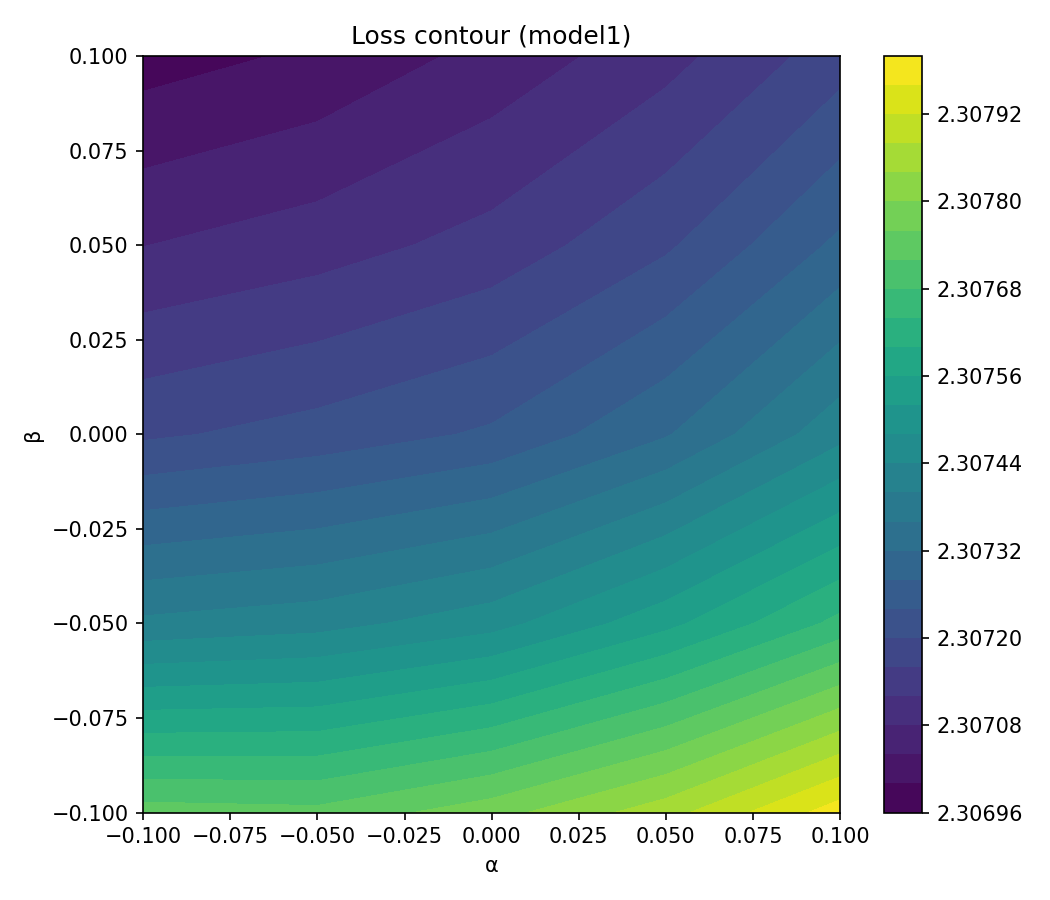
\includegraphics[width=0.85\textwidth]{figures/surface_contour_model1_r0.1.png}
    \caption{Контур исходной поверхности потерь при $r=0.1$.}
    \label{fig:surface_contour}
\end{figure}

\begin{figure}[H]
    \centering
    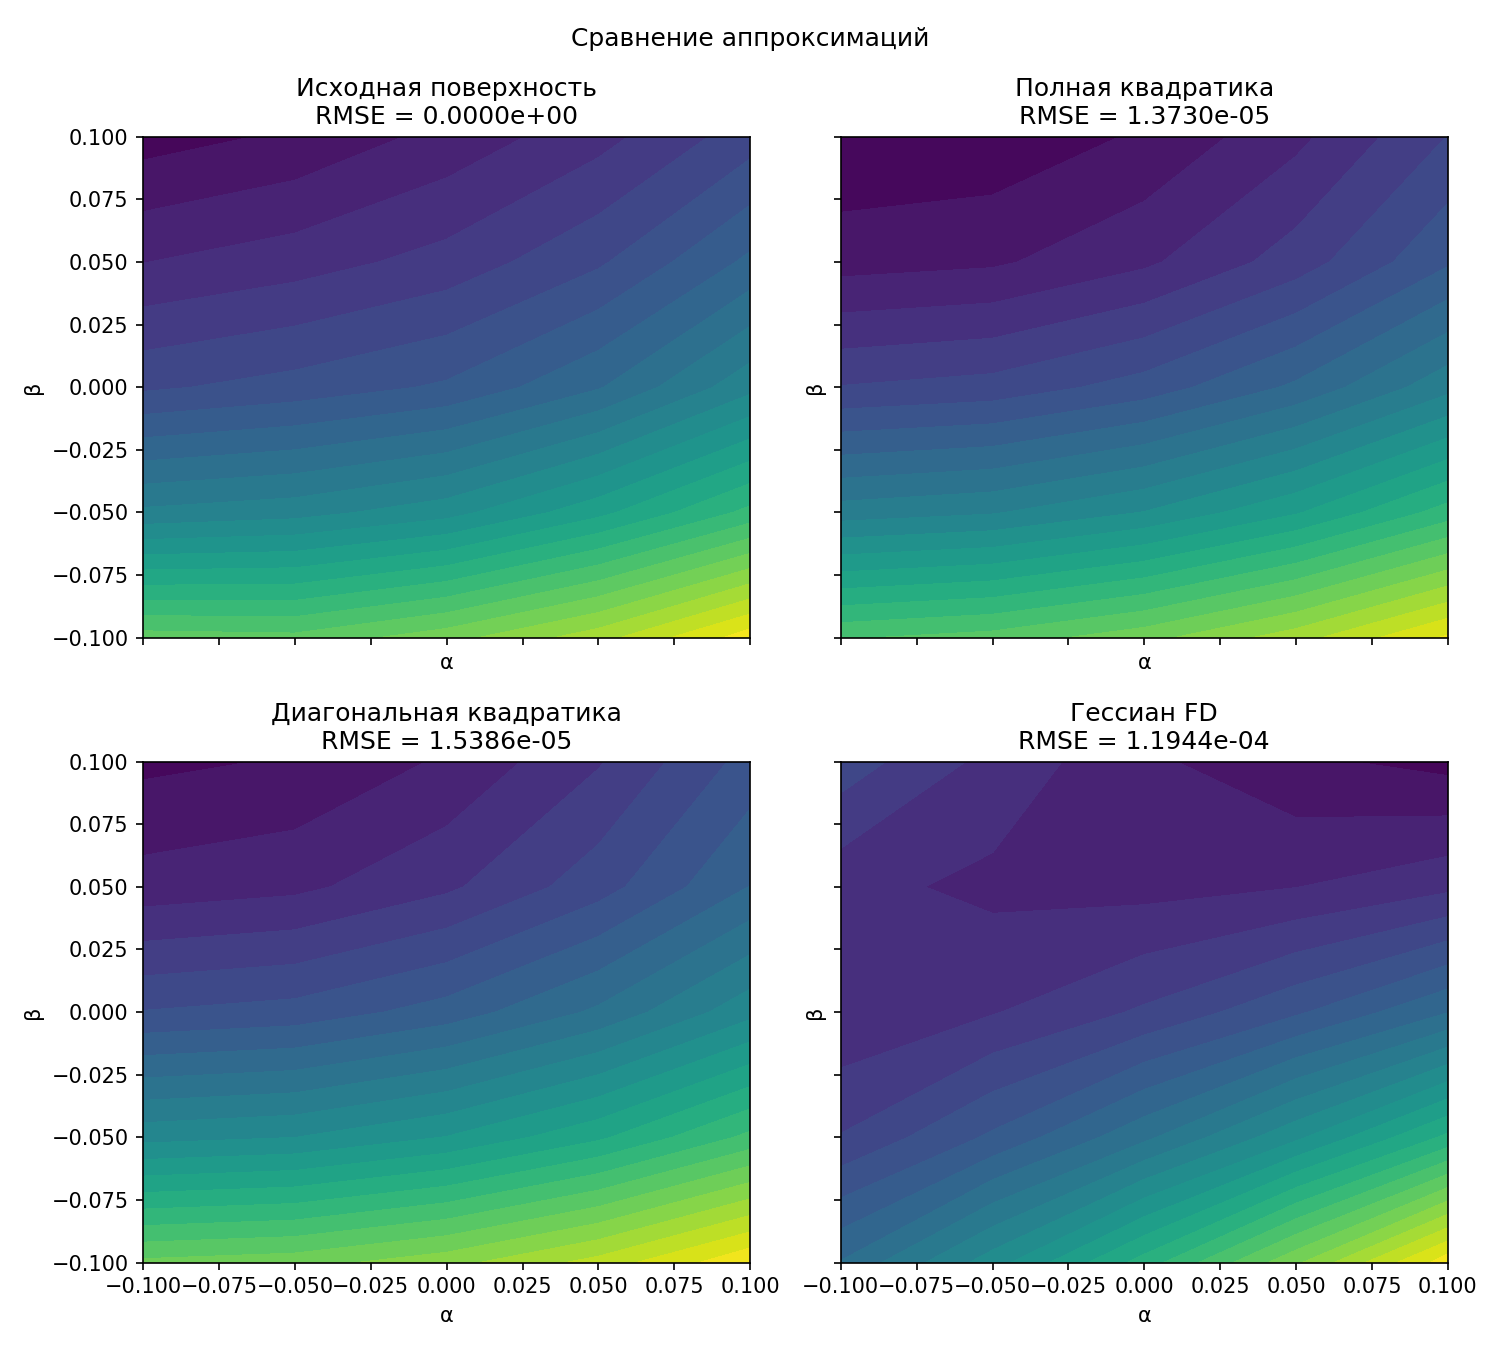
\includegraphics[width=0.85\textwidth]{figures/comparison_model1_r0.1.png}
    \caption{Сравнение исходной поверхности и аппроксимаций $q_1,q_2,q_3$.}
    \label{fig:surface_comparison}
\end{figure}

\begin{figure}[H]
    \centering
    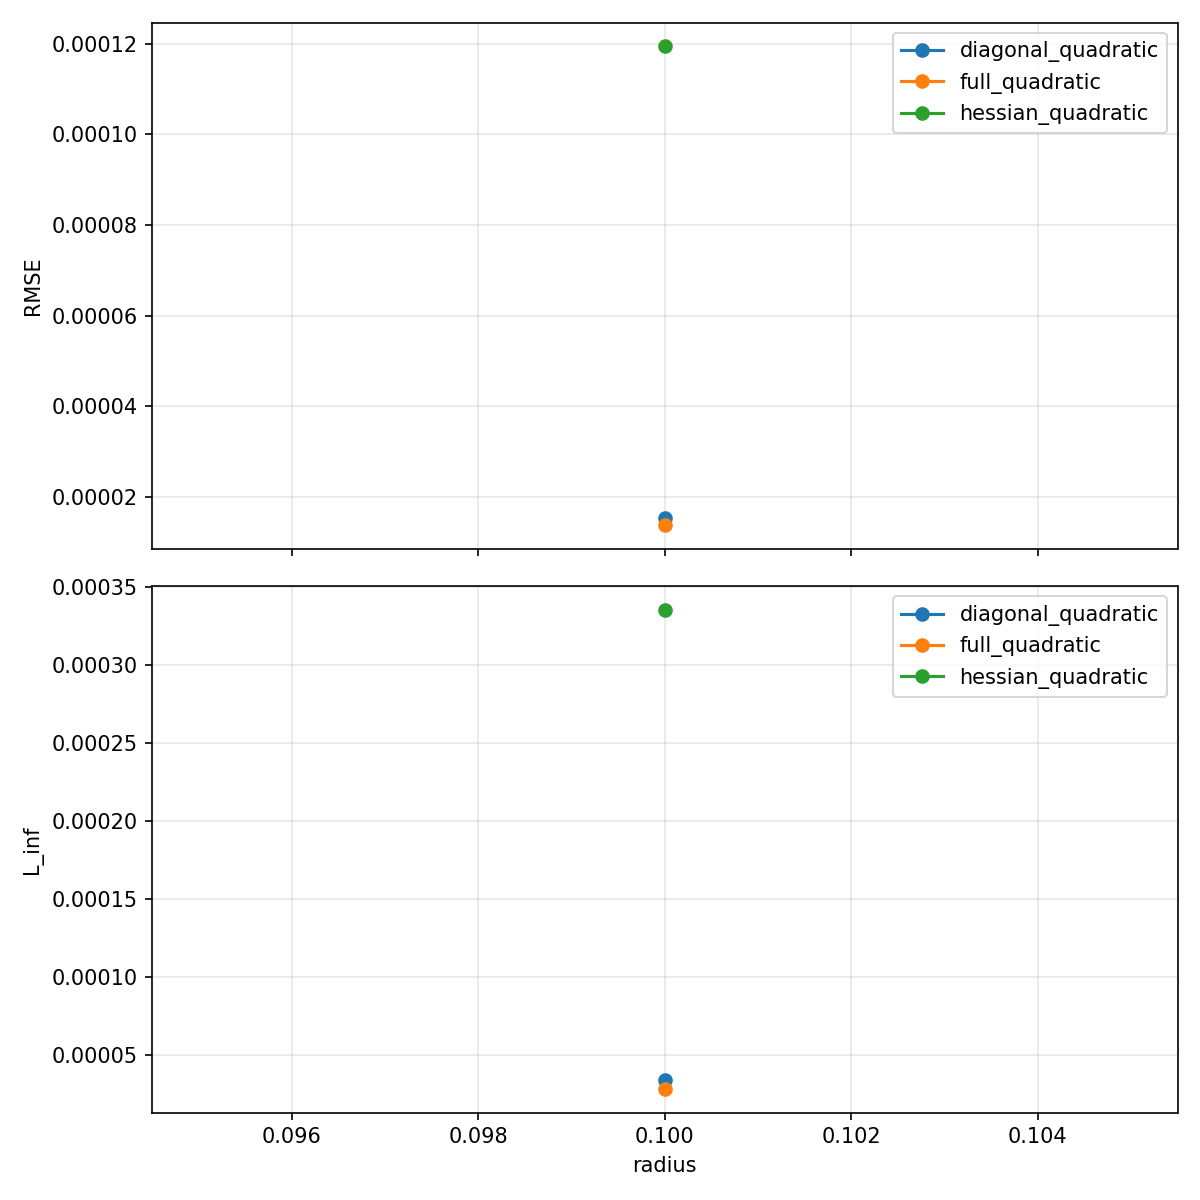
\includegraphics[width=0.85\textwidth]{figures/metrics_vs_radius_model1.png}
    \caption{Зависимость метрик аппроксимации от радиуса.}
    \label{fig:metrics_vs_radius}
\end{figure}

\section{Анализ результатов}

\subsection{Ключевые числа}
\begin{table}[H]
\centering
\begin{tabular}{lccc}
\toprule
Аппроксимация & RMSE & $L_\infty$ & RelRMSE \\
\midrule
full\_quadratic & 1.373e-05 & 2.814e-05 & 1.372e-02 \\
diagonal\_quadratic & 1.539e-05 & 3.401e-05 & 1.538e-02 \\
hessian\_quadratic & 1.194e-04 & 3.355e-04 & 1.194e-01 \\
\bottomrule
\end{tabular}
\caption{Метрики для model1 при $r=0.1$.}
\label{tab:metrics_r01}
\end{table}

\subsection{Интерпретация}
\begin{itemize}
    \item $q_1$ показывает наилучшее качество и подтверждает гипотезу о локальной квадратичности.
    \item $q_2$ близка к $q_1$, что говорит о малом вкладе смешанного члена в центре.
    \item $q_3$ заметно хуже: FD-оценка чувствительна к численному шуму и выбору шага $\epsilon$.
\end{itemize}

\subsection{Почему это научно важно}
Результат демонстрирует не просто «построение красивой картинки», а проверку гипотезы о структуре ландшафта с количественной валидацией.

\section{Дополнительный анализ}

\subsection{Direction sensitivity analysis}

Для сравнения направлений использовались варианты:
\begin{itemize}
    \item random + filter-normalized;
    \item layer-normalized;
    \item gradient-aligned;
    \item trajectory (TODO: недоступно из-за отсутствия промежуточных чекпоинтов).
\end{itemize}

\begin{table}[H]
\centering
\begin{tabular}{lcccc}
\toprule
Direction type & MAE & RMSE & RelRMSE & Relative L2 \\
\midrule
random\_filter\_normalized & 8.240e-05 & 1.093e-04 & 1.046e-01 & 4.740e-05 \\
layer\_normalized & 8.725e-05 & 1.152e-04 & 1.086e-01 & 4.996e-05 \\
gradient\_aligned & 2.959e-06 & 3.394e-06 & 1.483e-03 & 1.472e-06 \\
\bottomrule
\end{tabular}
\caption{Чувствительность качества квадратичной аппроксимации к выбору направлений.}
\label{tab:direction_sensitivity}
\end{table}

Градиентно-согласованное направление даёт наименьшую ошибку аппроксимации в эксперименте.

\subsection{Error scaling by radius}

Радиусы: $\{0.05, 0.1, 0.2, 0.3, 0.5\}$.
Оценена модель масштаба ошибки:
\[
\text{RMSE}(r) \sim C \cdot r^p,\quad p \approx 2.033.
\]

\begin{table}[H]
\centering
\begin{tabular}{lccc}
\toprule
Radius & MAE & RMSE & RelRMSE \\
\midrule
0.05 & 3.485e-05 & 4.520e-05 & 1.807e-02 \\
0.10 & 1.660e-04 & 2.131e-04 & 4.941e-02 \\
0.20 & 8.250e-04 & 1.039e-03 & 1.615e-01 \\
0.30 & 1.847e-03 & 2.287e-03 & 2.112e-01 \\
0.50 & 3.184e-03 & 4.332e-03 & 1.459e-01 \\
\bottomrule
\end{tabular}
\caption{Зависимость ошибки полной квадратичной аппроксимации от радиуса.}
\label{tab:error_by_radius}
\end{table}

\begin{figure}[H]
    \centering
    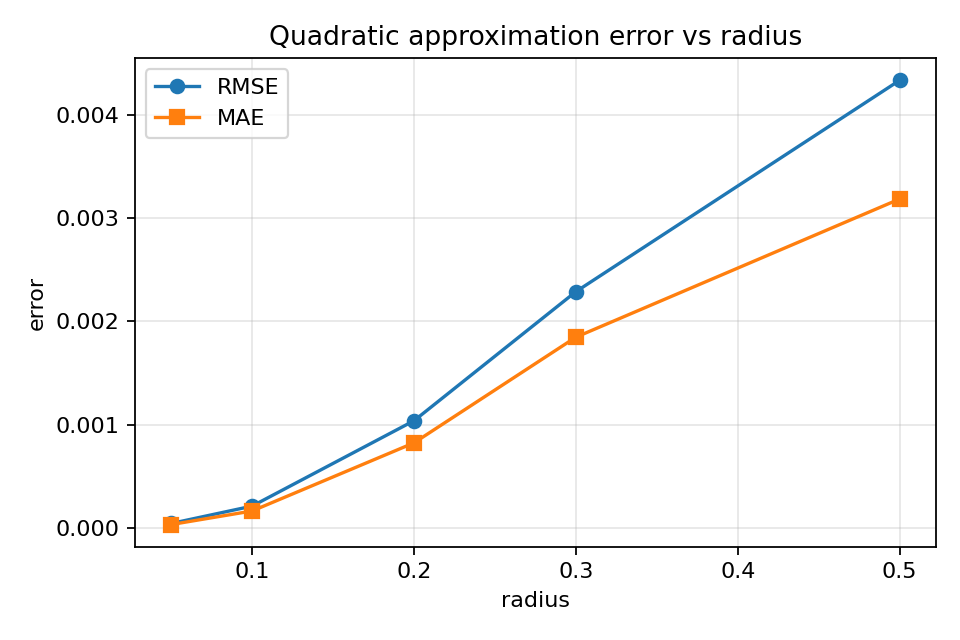
\includegraphics[width=0.72\textwidth]{figures/error_vs_radius.png}
    \caption{Error vs radius (linear scale).}
    \label{fig:error_vs_radius}
\end{figure}

\begin{figure}[H]
    \centering
    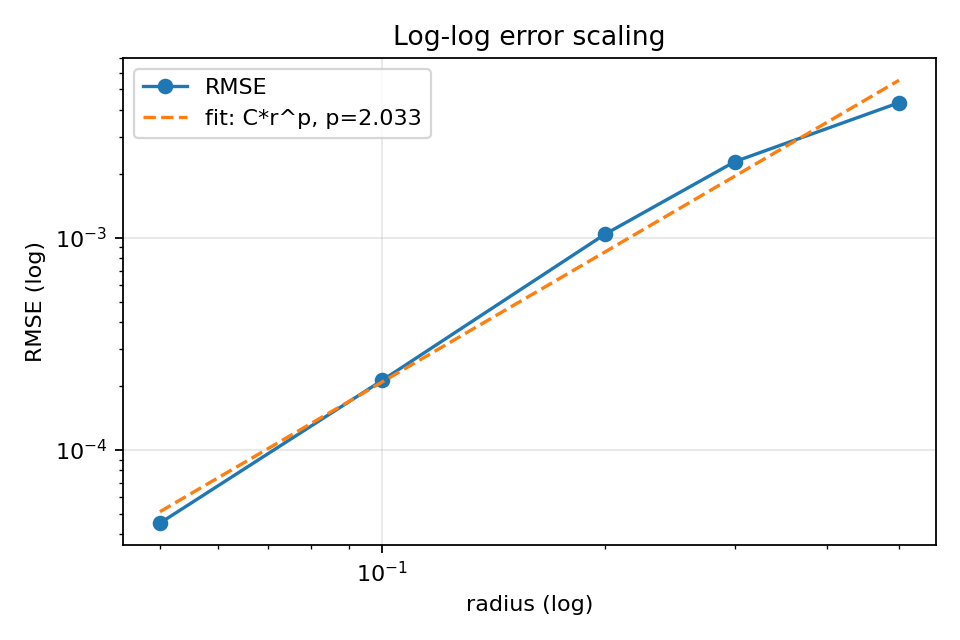
\includegraphics[width=0.72\textwidth]{figures/error_vs_radius_loglog.png}
    \caption{Error vs radius (log-log) и оценка показателя степени $p$.}
    \label{fig:error_vs_radius_loglog}
\end{figure}

\subsection{Training dynamics: flat vs sharp}

Для анализа динамики требуются checkpoint'ы ранних эпох. В текущем наборе артефактов присутствует только финальный checkpoint:
\begin{itemize}
    \item early (`epoch1`) --- TODO, отсутствует;
    \item middle (`epoch5`) --- TODO, отсутствует;
    \item final (`model1_final.pth`) --- доступен.
\end{itemize}

Для future-run в код обучения добавлена поддержка автосохранения checkpoint'ов `epoch1` и `epoch5`.

\begin{table}[H]
\centering
\begin{tabular}{lcccc}
\toprule
Checkpoint & $\lambda_{min}$ & $\lambda_{max}$ & Condition number & Sharpness \\
\midrule
final & 1.000e-06 & 1.000e-06 & 1.0 & 1.777e-03 \\
\bottomrule
\end{tabular}
\caption{Оценки кривизны и sharpness для доступного checkpoint.}
\label{tab:training_dynamics}
\end{table}

\begin{figure}[H]
    \centering
    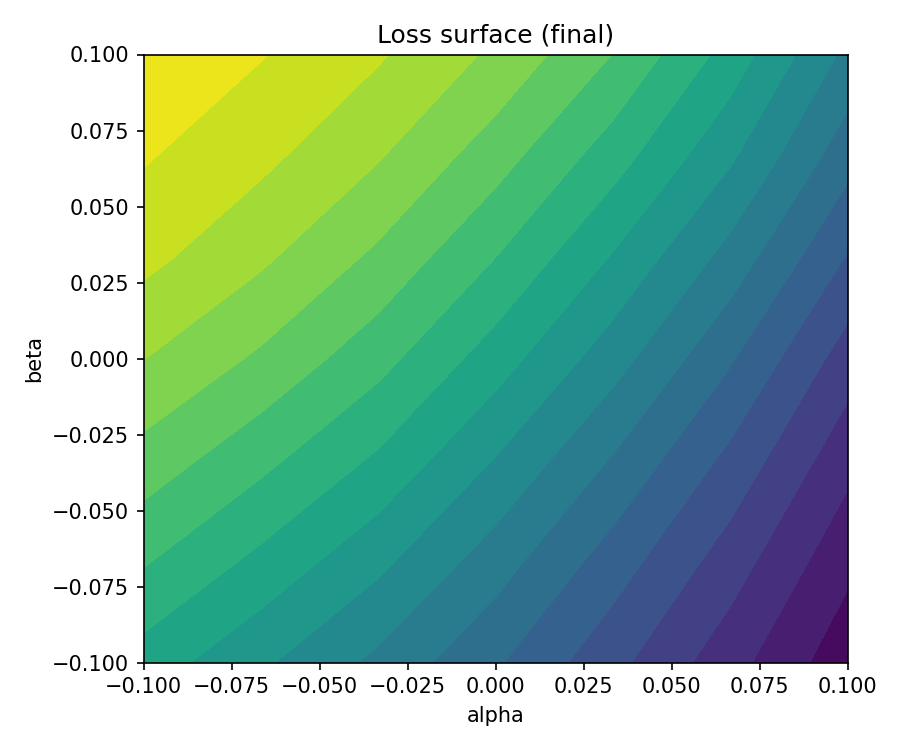
\includegraphics[width=0.72\textwidth]{figures/loss_surface_epoch_final.png}
    \caption{Loss surface для финального checkpoint.}
    \label{fig:loss_surface_final}
\end{figure}

\section{Сравнение конфигураций}

\subsection{Сравнение аппроксимаций}
\begin{itemize}
    \item \textbf{$q_1$ (full)}: лучшая точность, наиболее устойчивый baseline для этой задачи.
    \item \textbf{$q_2$ (diagonal)}: чуть хуже, но близка к $q_1$ и проще в интерпретации.
    \item \textbf{$q_3$ (FD Hessian)}: хуже на текущих настройках, требует отдельного sweep по $\epsilon$.
\end{itemize}

\subsection{Сравнение по осям 1D-среза}
\begin{figure}[H]
    \centering
    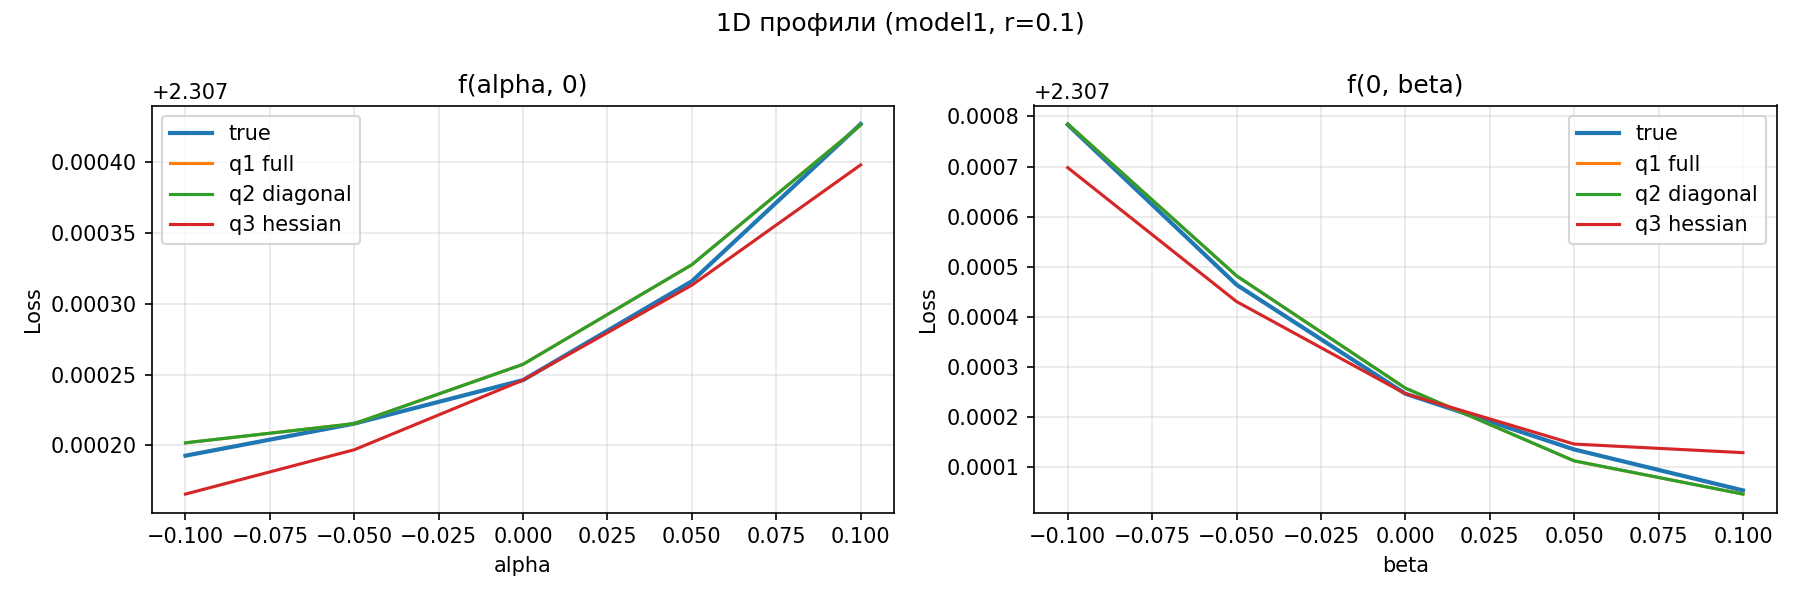
\includegraphics[width=0.9\textwidth]{figures/profile_1d_model1_r0.1.png}
    \caption{Срезы $f(\alpha,0)$ и $f(0,\beta)$ и их аппроксимации.}
    \label{fig:profile_1d}
\end{figure}

\subsection{Что не добавлялось сознательно}
Confusion matrix, ROC-кривые и другие классификационные визуализации не включены, поскольку они не являются центральными для цели ЛР (исследование геометрии loss landscape, а не сравнение классификаторов по precision/recall).

\section{Выводы}

\begin{enumerate}
    \item Построен воспроизводимый pipeline анализа loss landscape для CIFAR-10.
    \item Подтверждена гипотеза: в локальной окрестности решения полная и диагональная квадратики описывают поверхность лучше, чем FD-Hessian аппроксимация.
    \item Получены интерпретируемые связи между теорией (квадратичная локальная модель) и экспериментом (ошибки аппроксимации).
\end{enumerate}

\subsection{Ограничения}
\begin{itemize}
    \item Высокая стоимость полного прогона на CPU.
    \item Численная чувствительность FD-модели.
    \item Неполный набор сравнений по model2 в текущей версии отчёта.
\end{itemize}

\subsection{Следующие шаги}
\begin{itemize}
    \item Запустить системный sweep по $\epsilon$ для $q_3$.
    \item Добавить multi-seed анализ плоскостей $(d_1, d_2)$.
    \item Зафиксировать расширенную таблицу model1 vs model2 по всем радиусам.
\end{itemize}


\newpage
\bibliographystyle{plain}
\bibliography{bibliography}

\end{document}
